\documentclass[a4paper,12pt,times,numbered,print,index]{article}

\usepackage[italian]{babel}
\usepackage[utf8]{inputenc}
\usepackage{graphicx}
\usepackage{listings}
\usepackage{color}
\usepackage{fancyhdr}
\usepackage[margin=1in]{geometry}
\usepackage{hyperref}
\usepackage[backend=biber, style=authortitle-comp]{biblatex}
%
% File della bibliografia
%
\addbibresource{bibliografia.bib}

%
% Impostazioni per head e foot
%
\pagestyle{fancy}
\fancyhead{}
\fancyfoot{}
\fancyhead[R]{Designer}
\fancyfoot[L]{\thepage}
\fancyfoot[R]{\slshape{\footnotesize{Guglielmo Bartelloni - Francesco Bellezza}}}

%
% Impostazioni per link dell'indice
%
\hypersetup{
    colorlinks,
    citecolor=black,
    filecolor=black,
    linkcolor=black,
    urlcolor=black
}

% Colori per inserire syntax highlight
\definecolor{dkgreen}{rgb}{0,0.6,0}
\definecolor{gray}{rgb}{0.5,0.5,0.5}
\definecolor{mauve}{rgb}{0.58,0,0.82}

% Setting per Java

\lstset{frame=tb,
  language=Java,
  aboveskip=3mm,
  belowskip=3mm,
  showstringspaces=false,
  columns=flexible,
  basicstyle={\small\ttfamily},
  numbers=none,
  numberstyle=\tiny\color{gray},
  keywordstyle=\color{blue},
  commentstyle=\color{dkgreen},
  stringstyle=\color{mauve},
  breaklines=true,
  breakatwhitespace=true,
  tabsize=3
}
\author{Guglielmo Bartelloni}
%
% Inizio del documento
%
\begin{document}
%
% TITOLO
%
\begin{titlepage}
\begin{center}
	\vspace{1cm}
	\textbf{\huge{Designer}}\\ 
	\vspace{1cm}
	
\includegraphics[scale=0.7]{logoITTS.jpg}\\
	\vspace{1cm}
	\large{Guglielmo Bartelloni, Francesco Bellezza}\\
	\vspace{0.5cm}
	24 Dicembre, 2017\\
	\today\\
	\vspace{0.5cm}
	\vspace{0.5cm}
	4IB\\
	Luigi Vestri e Davide Caramelli\\
	\vspace{1cm}
	\Large{Laboratorio di Informatica}
\end{center}
\end{titlepage}
\vspace*{1cm}
\tableofcontents
\clearpage
%
% Inizio del CORPO
%
\section{Scopo dell'esercitazione}
Lo scopo dell'esercitazione e quella di realizzare un programma che consenta di disegnare figure geometriche e grafici di funzioni permettendo di salvare le figure sul un file di testo.

\section{Cenni Storici}


\subsection{Ereditarieta'}
L’ereditarietà è una relazione di tipo is-A, dove una superclasse mette a disposizione di una sottoclasse i suoi metodi e attributi non privati (a eccezione del costruttore).

In Java, per estendere una superclasse e per creare quindi la sottoclasse, si utilizza la parole chiave extends accanto al nome della sottoclasse e accanto alla parola extends si inserisce il nome della superclasse.

Nel caso delle interfacce, ovvero particolari classi che al loro interno contengono solamente metodi astratti, si utilizza la parola chiave implements.
\textcite{corsoinformatica}

\subsection{Polimorfismo}
Il polimorfismo è una tecnica che consente di utilizzare metodi polimorfici, ovvero metodi che hanno lo stesso nome, ma implementazioni diverse.
Esistono due tipi di polimorfismi principali: per overloading e per overriding.

Nel polimorfismo per overloading si opera a un livello locale, ovvero all’interno di una classe.

Il metodo polimorfico in questo caso deve:
\begin{itemize}
	\item Avere lo stesso nome degli altri metodi polimorfici.
	\item Avere numero di parametri diversi o avere tipi di parametri diversi o avere ordine di parametri diversi rispetto agli altri metodi polimorfici.
	\item Può avere un tipo di ritorno diverso se i due punti qua sopra sono rispettati.
\end{itemize}
Nel polimorfismo per overriding si opera a un livello di superclassi e sottoclassi.

Nelle sottoclassi viene ridefinito il metodo presente nelle superclassi.

Il metodo polimorfico in questo caso deve:
\begin{itemize}
	\item Avere la stessa signature del metodo della superclasse.
	\item Avere lo stesso tipo di ritorno della superclasse o un sottotipo del tipo di ritorno della superclasse (stesso discorso vale per i parametri).
	\item I metodi private non vengono ereditati alla classe figlia, quindi non si può effettuare l’overriding del metodo.
	\item Le clausole come native, strictfp possono essere incluse nel metodo della classe figlia.
	\item Un metodo statico può essere solo adombrato e non sovrascritto.
\end{itemize}
\textcite{polimorfismo}


\section{Analisi Funzionale}


\subsection{Ipotesi Risolutiva}
Il programma deve riuscire a disegnare figure elementari su un pannello. Per farlo viene utilizzato l`oggetto graphics andando a reimplementare la classe 
\begin{lstlisting}
public void paintComponent(Graphics g);
\end{lstlisting}

\subsection{Funzionalitá del programma}
Le funzionalitá che si devono implementare sono:
\begin{enumerate}
	\item Salvare su file
	\item Caricare da file
	\item Disegnare figure(quadrato, arco, linea, ellisse, rettangolo, grafico, cerchio e ellisse)
	\item Disegnare Font(grandezza, tipo,  stile)
\end{enumerate}

L`interfaccia si presenta in questo modo:


\section{Analisi Tecnica}

\subsection{Scomposizione Top-Down}

\subsection{UML}
\begin{center}
	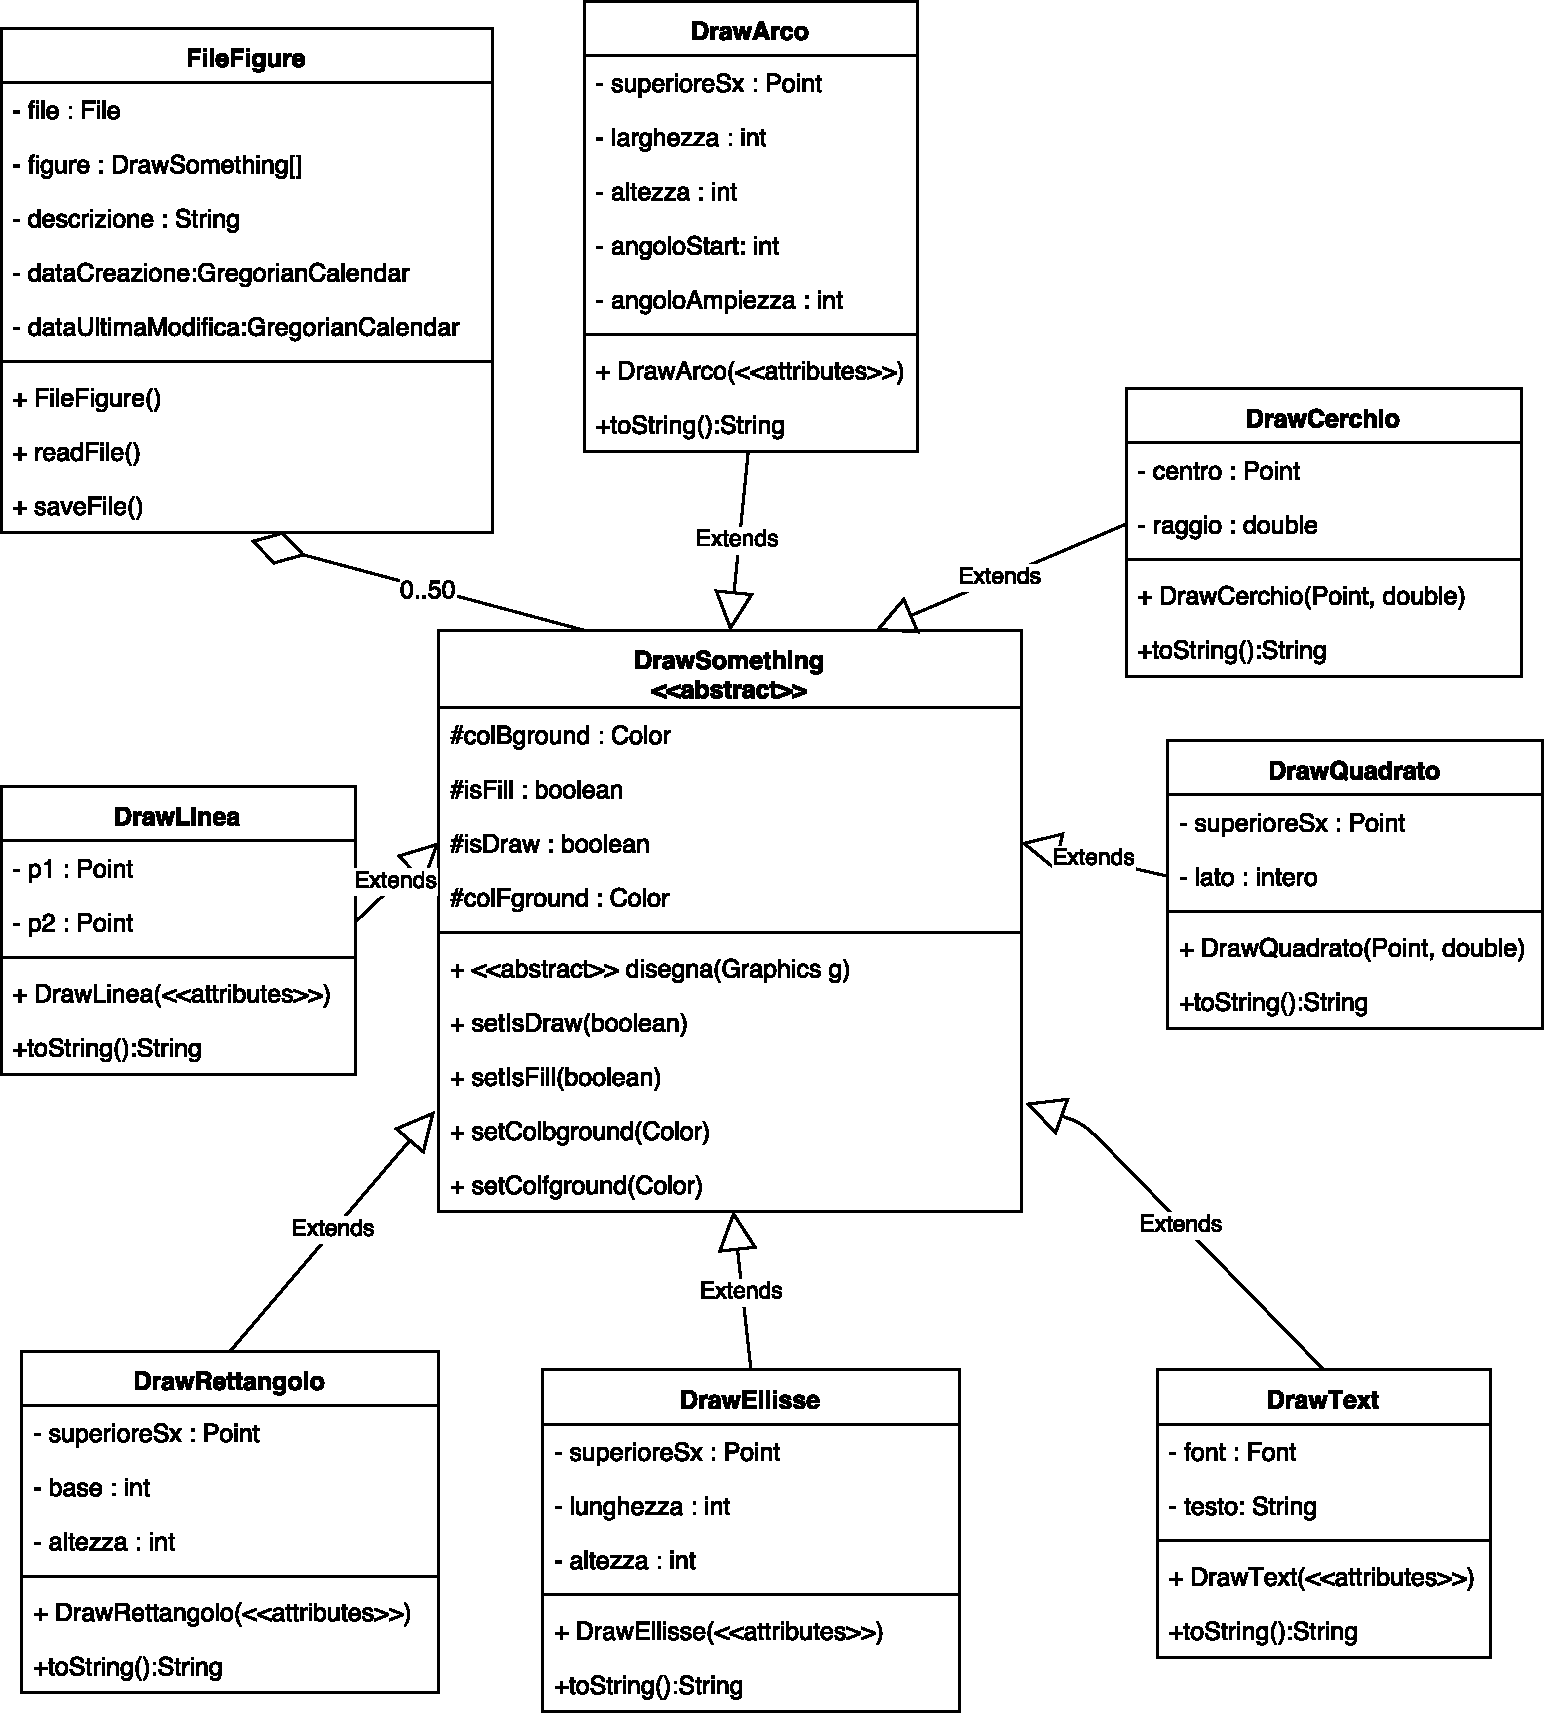
\includegraphics[scale=0.4]{Immagini/UML.pdf}
	\label{UML}
\end{center}


\subsection{Descrizione Classi}
\subsubsection{MainFrame} %Nome della classe 
\subsubsection{DrawSomething} %Nome della classe
La classe \textit{DrawSomething} é una classe astratta che dichiara alcuni metodi per impostare i colori e un metodo astratto per essere riscritto nelle classi figlie.
É pensata all'unico scopo di essere estesa dalle altre classi \textit{draw} che implementeranno il metodo \textit{toString()} e il metodo \textit{draw(Graphics g)} come mostrato in figura \ref{UML}.
Gli attributi di questa classe sono i seguenti:
\begin{lstlisting}
protected Color colBground;
protected Color colFground;
protected boolean isFill;
protected boolean isDraw;
\end{lstlisting}
\subsubsection{FileFigure}
La classe \textit{FileFigure} é la classe che si occupa di gestire di gestire il ripristino e il salvataggio delle figure nel file di testo.

Il metodo \textit{readFile()} si occupa di leggere il file di testo e salvare le figure nell'array.

Il metodo \textit{saveFile()} si occupa di salvare l'array di figure all'interno del file di testo. Per il salvataggio delle figure viene utilizzato il metodo \textit{toString()} di ogni figura.


\section{Test Data Set/Debug}

\printbibliography
\end{document}
